In this section we highlight how the UC experiment is encoded in NomosUC by \msf{execUC}.
Recall from Section~\ref{sec:basic} that linear session types impose constraints on what forms of communication can be captures, and pose challenges to supporting 
a dynamic number of protocol parties, or functionalities, at runtime. 
We detail how our encoding realizes dynamic parties through the use of virtual tokens in our \partywrapper, and validated our encoding by realizing a few critical results from the UC literature: the Dummy Lemma, a composition operator, and a multisession operator. 
These three results allow us to ultimately conclude that NomosUC realizes full UC composition.

%Combined with providerless channels, we create the \partywrapper that runs protocol parties in a sandbox and manages their communication with \F, \A, and \Z.
%We validate our encoding of the UC experiment by realizing a critical result from the UC literature, the Dummy Lemma, which highlights the degree to which NomosUC captures the flexibility and modularity of the UC ITM model. 
%Finally we cover to important operators, composition and multisession, which allow us to prove the full composition theorem of UC in NomosUC.


\subsection{The UC Experiment}
%The UC experiment is an execution of protocol parties and an ideal functionality, reacting to input by an adversary \A or the environment \Z.
The UC experiment is instantiated by the \msf{execUC} function. 
It's definition is straightforward owing to our use of providerless channels. 
\m{execUC} is parameterized by at least one virtual token type to allow for sandboxing (usually by the adversary or environment) and message type parameters specified for the protocol in question. 
It additionally takes in a security parameter $k$ and a random bit string $r$ that is used as a source of randomness for all future processes. 
{\centering
\parbox{0cm}{
\begin{tabbing} 
 $\m{execout}[a] = \textcolor{red}{\getpot^n} \echoice{\mb{exec}: $\=$ \ichoice{ \mb{out}: Bit \product 1}}$ 
 \end{tabbing}}
}

Its type $\m{execout}[a]$ accepts $n$ import tokens, and returns an output \inline{Bit} as the result from \Z. 
The NomosUC type system requires explicit polynomials for checking runtime bounds, and this allows us to ensure runtime that is $poly(k)$ as long as the the number of tokens $n \in poly(k)$.

All main processes in NomosUC are wrapped according to the providerless channel specification in Section~\ref{sec:basic}. 
Therefore, \m{execUC} creates only the shared parts of the providerless channel and passes them as input to the wrapped processes. For example \Z and \A are connected by the following channels: parameters to both \A and \Z. 
%\begin{figure*}
%\begin{lstlisting}[basicstyle=\footnotesize\BeraMonottFamily, mathescape, frame=single]
%$\nproc$ execUC[K][p2f,f2p][z2p,p2z][a2p,p2a][f2a,a2f]{p2fn,f2pn}{z2pn,p2zn}{a2pn,p2an}{f2an,a2fn}{n}: 
%  (k: Int), (rng: [Bit]) |- ($\$$d: execout)
%\end{lstlisting}
%\caption{Type definition for \m{execUC} with no virtual tokens.}
%\label{fig:execuc}
%\end{figure*}
\begin{lstlisting}[basicstyle=\footnotesize\BeraMonottFamily, mathescape]
#z_to_a $\leftarrow$ channel_init[$\tp{K}$][$\tp{z2a}$]{$\tp{z2an}$}
#a_to_z $\leftarrow$ channel_init[$\tp{K}$][$\tp{a2z}$]{$\tp{a2zn}$}
$\tg{...}$
$\$$z <- Env[K] k rng #z_to_p #p_to_z #z_to_a #a_to_z ;
\end{lstlisting}
The type parameters to the channels are the token type \inline{K} and some of the message / import type paraeters to \m{execUC}.
%When processes are spawned, their shell codes correctly connect the channel endpoints internally.
%We point out that process definitions for \Z, \A, \F, and $\Pi$ are not passed as parameters to \inline{execUC} because NomosUC currently doesn't support passing them as parameters.

\paragraph{Execution Parameters}
The environment, \Z, is the first spawned process and defines the main parameters for the rest of the execution: the session ID and the set of corrupted parties.  
According to its type \m{EtoZ} (below), \Z sends the SID (a user-defined type) and the corruption list to \m{execUC} that passes them to \F, \A and the \partywrapper.  
\Z starts on input \mb{start} with $n$ tokens. 
{\centering
\parbox{0cm}{
\begin{tabbing}
 $\m{EtoZ}[a] = \textcolor{red}{\getpot^n} \ichoice{\mb{init}: $\=$ SID[a] \arrow [PID] \arrow$ \\
\>$\echoice{\mb{start} \arrow \ichoice{\mb{out}: Bit \arrow 1}}}$
 \end{tabbing}}
}
Finally, the output bit, \Z's guess of which world it is in, forms the basis of the definition of indistinguishability.

%\begin{figure*}[t]
%\begin{lstlisting}[basicstyle=\scriptsize\BeraMonottFamily, frame=single, mathescape, caption={The process definition of the \msf{execUC} function.}]
%$\Stype$ Bit{n} = <{n}| &{ exec: +{out : Bit $\rightarrow$ 1}} ;
%
%$\tb{proc}$ execUC[$\tp{K}$][$\tp{K1}$][$\tp{sid}$][$\tp{p2f,f2p}$][$\tp{z2p,p2z}$][$\tp{a2p,p2a}$][$\tp{a2f,f2a}$]{$\tp{p2fn,f2pn}$}{$\tp{p2zn,z2pn}$}{$\tp{a2pn,p2an}$}{$\tp{a2fn,f2an}$} :
%  (k: $\tgr{int}$), (r: [Bit]) |- ($\$$d: Bit)
%\end{lstlisting}
%\label{lst:execuc}
%\end{figure*}

\subsection{The \partywrapper}
\begin{figure}
	\centering
	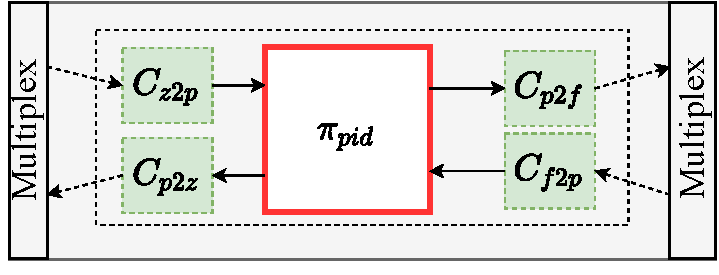
\includegraphics[scale=0.5]{figures/singleshellmultiplex.pdf}
	\caption{This is the \partywrapper that routes messages to the correct internally runnint protocol party. This figure shows how one protoco party (dotted box) is instantiated within it. The party $\pi_{pid}$ is shell code akin to Figure~\ref{fig:newpandq}.}%\snote{Updated caption to say it's multiplexer with one instance. The reason I don't want to include another instance is that I couldn't figure out a way to add it and expand the diagram horizontally. It will leave so much white space on the sides if I add a new party and will take up much more vertical space which we need to cut down on anyway.}}
	\label{fig:singlemultiplex}
	\vspace{-3mm}
\end{figure}
We use the \partywrapper to handle spawning parties, creating their channels, and connectint them to the rest of the experiment.
Instead of parties directly connected to \F and \Z through a providerless channels, the \partywrapper runs them virtually and presents a consistent ``real'' view to them. 
Virtual tokens enables the types and import requirements of the protocol parties to be met while sandboxing them. 
The \partywrapper, in turn, is connected by single channels to \F, \Z, and \A, and it routes communication to/from the appropriate protocol party. 
In Figure~\ref{fig:singlemultiplex}, we see a wrapped protocol party, with its generated processes, inside the \partywrapper. \todo{this figre now just looks like an example of a wrapped process and not to insightful}

The \partywrapper design implies that the import sent to it by \F, \Z, and \A must be constant, because they each communicate with it over a single providerless channel. However, the protocol parties still receive and operate on virtual tokens according to their type. 
We don't see this as a downside of the approach as tight runtime constraints are not an intended goal of NomosUC or the UC framework.

The \partywrapper forces \F to also be wrapped to multiplex communication from the \partywrapper. 

\subsection{Emulation}
The central security definition in UC is indistinguishability between the real and ideal world experiments.
We define indistinguishability in terms of the ensemble of distributions created by the output bit of the partial term $\m{execUC}\ \pi\ \F$ over all possible bitstrings and security parameters. 
We sa that two worlds are indistinguishable if $\forall \A\ \exists \Sim\ \forall Z$ the ensembles have  \emph{statistical difference} that is negligible in $k$ (Definition~\ref{def:emulation}).

%We define the output bit of the partial term of \inline{execUC}, for a specific $\pi$ and \F, as an ensemble of distributions over all possible random bitstrings and security parameters.
%Emulation, then, is about the ensembles created by two UC executions being computationally indistinguishable from each other.
%We define indistinuishability between ensembles in a standard way using \textit{statistical distance}: $\mathcal{D}_{1,k} sim \mathcal{D}_{2,k}$ if their statistical distance is at most $negl{k}, \forall k$.
%\begin{definition}[Indistinguishability]\label{def:distance}
%Two ensembles $\mathcal{D}_{1,k}, \mathcal{D}_{2,k}$ are indistinguishable, $\mathcal{D}_{1,k} \sim \mathcal{D}_{2,k}$, if their statistical distance is at most $negl(k), \forall k$.
%\end{definition}

\begin{definition}[Emulation]\label{def:emulation}
If two protocols $(\pi, \F_1)$, $(\phi, \F_2)$, which we refer to only by \PI and $\phi$, emulated each other, then $\forall \A$ of type $\Delta_3'$ well-matched with \PI, there must $\exists \Sim$ of the same type,  well-matched with $\phi$, s.t. $\forall \Z$ : $\msf{execUC}(\pi, \F_1, \Z, \A)$ $\approx$ $\msf{execUC}(\phi, \F_2, \Z, \Sim)$:

\begin{mathpar}
	\footnotesize
	\inferrule*[right=emulate]
	{
		\pi : \Delta_1'[\Tokentypes][\mathrm{T}_{\pi}] \semi \phi : \Delta_2'[\Tokentypes][\mathrm{T}_{\phi}] \semi \\
		\forall \A \ | \ \Delta_4[\Tokentypes][\mathrm{T}_{\A}] \vdash \A :: \Delta_3', \ \langle \A \leftrightarrow \pi \rangle \\
		\Rightarrow \exists \ (\Delta_3[\Tokentypes][\mathrm{T}_{\Sim}] \vdash \Sim_\A :: \Delta_3') \ | \ \langle \Sim_\A \leftrightarrow \phi \rangle \\
		\Rightarrow \forall \Z  \; \msf{execUC} \ \pi\ \F_1\ \Z\ \A \approx\ \msf{execUC} \ \phi\ \F_2\ \Z\ \Sim_\A
	}
	{
		% EMULATION DEFINITION
		\lambda \A \, . \, \Sim_\A \vdash (\pi, \F_1) \sim (\phi, \F_2)
	}
\end{mathpar}
\end{definition}
The notation $e \leftrightarrow e'$ is used to denote two \emph{well-matched} terms: a configuration connected the two is well-typed. 

\subsection{Evaluation}
An important validation of our approach is the the Dummy Lemma~\ref{thm:dummythicclemma} which shows that a simulator, \DS, for the dummy adversary, suffices to prove emulation. 
\begin{theorem}[Dummy Lemma]\label{thm:dummythicclemma}
If \ $\exists \DS$ s.t. $ \DA, \DS \vdash \F_2 \xrightarrow{\pi} \F_1$ then $\forall \A \ \exists \Sim_\A$ s.t. $\Sim_{\A} \vdash  \F_2 \xrightarrow{\pi} \F_1)$ 
\end{theorem}
The proof of the Lemma is in the form of systematic constructor for a simulator for any arbitrary real world \A (in Appendix~\ref{sec:dummy}.
Though a simple Lemma, the simplicity of the resulting simulator proof highlights the simplicity and expressiveness that our token heirarcy and sandboxing afford. 

\subsection{Single Composition}
In this section we present a composition operator for protocols that completes Theorem~\ref{thm:singlecomp}.

The composition allows replacement of a single ideal functionality $\F_2$ with a protocol $\pi$ that realizes it in the $\F_1$-hybrid world. 
A protocol party $\rho_i$ that gives input to $\F_2$ instead gives input to party $\pi_i$. 
The composes protocol $\rho \circ \pi$ connects parties of both protocols with providerless channels in the \partywrapper. 
%In NomosUC, composition of protocols occurs in the \partywrapper where output from $\rho_i$ to $\F_2$ is given as input to $(\pi, \F_1)$. $\pi$ runs in the \partywrapper and $\F_1$ is the hybrid functionality. 
%The operator connects parties of $\rho$ and $\pi$ through providerless channels where $\rho$ gives input to $\pi$. 
Like \m{execUC} (whose code can be seen in the Appendix), the operator operates on wrapped processes. That means it spawns the shared providerless channels and connects the wrapped processes.
\begin{lstlisting}[basicstyle=\footnotesize\BeraMonottFamily, mathescape, frame=single]
#rho2pi $\leftarrow$ channel_init[K][rho2f]{rho2fn} ;
#pi2rho $\leftarrow$ channel_init[K][f2eho]{f2rhon} ;

$\$$r $\leftarrow$ rho <- k rng sid pid #z2p #p2z #rho2pi #pi2rho; 
$\$$p $\leftarrow$ pi <- k rng sid pid #rho2pi #pi2rho #p2f #f2p;
\end{lstlisting}

%Recall that every protocol and functionality comes with generated processes which handle communication as part of the providerless channels as depicted in Figure~\ref{fig:newpandq}.
%In the code snippet above, this means that \inline{rho} and \inline{pi} are wrappers that encapsulate the actual protocol and the generated processes, and passing the channel endpoints to the shell connects them correctly. 

%The processes \inline{rho} and \inline{pi} are actually wrapped processes like the one depicted in Figures~\ref{fig:newpandq} and \ref{fig:singlemultiplex}.
%The challenge in creating a generic composition operator is managing protocol and type-specific providerless channels.  
%As we stated previously, the \partywrapper and protocol channels rely on some code generation in order to make use of expressive session types, and the composition operator is now different.
%In our construction above, 

%The generic composition operator of NomosUC connects the shells of parties $\rho_i$ and $\pi_i$ through providerless channels. 
%As mentioned earlier, for functionalities/protocols that don't need to split communication over two channels, the coposition operator can be trivialized by directly connected the channel offered by $\rho_i$ as the input channel of $\pi_i$.
%The type system here guarantees that our composition gives $\pi_i$ an appropriate amount of import and tha the resulting protocol is also polynomially bound. 

Part of the security proof of security under composition is providing a simulator that ensures emulation.
For this we can define simulator compostion operator that connects the simulators \SIM{\rho} and \SIM{\pi} in same way as the Dummy Lemma: \SIM{\pi} receives input from \Z and \SIM{\rho} receives output fro m \F and the \partywrapper.

\subsection{UC Composition}

\begin{theorem}[Composition]\label{thm:composition}
\begin{mathpar}
\inferrule*[right=compose]
{
	%(\pi, !\F_1) \sim (\idealP, F_2) \semi (\rho, !\F_2) \sim (\idealP, \F_3) \\ 
	!\F_1 \xrightarrow{\pi} \F_2 \semi !\F_2 \xrightarrow{\rho} \F_3 \\
	%\Rightarrow \exists \Sim(\A) \vdash (\rho^{!\F_2 \rightarrow (!\pi \, \circ \, \msf{squash})}, !\F_1) \sim (\idealP, \F_3)
}
{
	!\F_1 \xrightarrow{\rho \, \circ !\pi \circ \, \msf{squash}} \F_3
	%(\rho \, \circ \, !\pi \circ \msf{squash}, !\F_1) \sim (\idealP, \F_3)
}
\end{mathpar}
\end{theorem}

Full composition, Theorem~\ref{thm:composition}, extends Theorem~\ref{thm:singlecomp} to replace multipe concurrent instances of a functionality with a realizing protocol.
We show that it can be realized in NomosUC by first introducing  an operator $!$ and intermediate Theorems~\ref{thm:functor} and \ref{thm:squash}. We cover the latter in the appendix
because it's statement and proof are intuitive. 
\begin{theorem}[Multisession Composition]\label{thm:functor}
	\begin{mathpar}
		\inferrule*[right=MultiComp]
		{
			\F_1 \xrightarrow{\pi} \F_2
		}
		{
			!\F_1 \xrightarrow{!\pi} !\F_2
		}
	\end{mathpar}
\end{theorem}
Theorem~\ref{thm:functor} is easily proven by replicating the single simulator because the concurrent sessions don't share any state. We describe the simulator in the Appendix, and, again we rely on our novel virtual tokens construction to implement it. 
Defining these extensions, theorem and their simulators in NomosUC allows us to conclude that NomosUC captures the full, generlized UC composition theorem with the following argument. 

\begin{proof}
By Theorem~\ref{thm:singlecomp} we have that $\F_1 \xrightarrow{\pi} \F_2$. If we combine this result with Theorem~\ref{thm:functor} we can conclude that $!!\F_1 \xrightarrow{\rho \circ !\pi} !\F_3$. 
Finally we can squash two $!!$ operators into one $!$ with Theorem~\ref{thm:squash} (in Appendix~\ref{app:ms}) to get $!\F_1 \xrightarrow{\rho \circ !\pi \circ \m{squash}} \F_3$.
\end{proof}

The relative simplicity of our encoding of the UC experiment, the related opreators and theorems, comes down to our providerlss channel abstraction that removes constraits on possible communication patterns, the virtual token heirarchy that allows re-use of code akin to the UC ITM model of computation, and a strong type system that guarantees us polynomial time execution.

